\documentclass{beamer}
\usepackage[brazil]{babel}
\usepackage[utf8]{inputenc}

\usepackage{amsmath}
\usepackage{amsfonts}
\usepackage{amssymb}
\usepackage{makeidx}
%\usetheme{Warsaw}
\usetheme{CCNU}

\title{Variáveis e Constantes}
\subtitle{Variáveis e Constantes}
\author{Pedro Lima}
\institute{PLmatemática}
\date{2022}

\begin{document}
    % Slide 1
    \maketitle
    
    % Slide 2
    \begin{frame}{Introdução}
        \begin{center}
            
\includegraphics[width=3cm]{imagens/images.png}
        \end{center}
        \begin{block}{O que são os conjuntos numéricos?}
            São grupos de números que contém certas características.
        \end{block}
    \end{frame}
    
    % Slide 3
    \begin{frame}{Naturais ($\mathrm{N}$)}
        $\mathrm{N} = 0, 1, 2, 3, ... , +\infty$\\
        $x \in \mathrm{N}$ $|$ $x \ge 0$\\
        \begin{alertblock}{Naturais positivos}
            $\mathrm{N}^* = \mathrm{N} - \{0\}$\\
            $x \in \mathrm{N}$ $|$ $x > 0$
        \end{alertblock}
        \begin{block}{Característica}
            O conjunto dos naturais é o grupo de números positivos e/sem o número nulo.
        \end{block}
        \begin{block}{Origem}
            Surgiu de forma simples como contar nos dedos, por isso o nome "natural", incorporando a ideia de ter algo. O zero também surgi de forma natural como deixar os dedos abaixados.
        \end{block}
    \end{frame}
    
    % Slide 4
    \begin{frame}{Inteiros ($\mathrm{Z}$)}
        $\mathrm{Z} = -\infty, ...,-2,-1, 0, 1, 2, ..., +\infty$
        \newline
        \begin{block}{Característica}
            Observe que $\mathrm{Z_+} = \mathrm{N^*}$ e $\mathrm{Z_+} +\{0\} = \mathrm{N}$.\\
            O conjunto dos inteiros contém o grupo dos naturais e seu oposto.\\
            Ex.: O número 1 é oposto do número -1.
        \end{block}
        \begin{block}{Origem}
            Vem da concepção de dever ou pagar algo. Se estou em dívida então tenho $-x$ de dinheiro.
        \end{block}
    \end{frame}
    
    % Slide 5
    \begin{frame}{Racionais ($\mathrm{R}$)}
        $\mathrm{Q} = -\infty, ..., -\frac{1}{1}, -\frac{1}{2}, ..., 0, ..., \frac{1}{2}, \frac{1}{1}, ..., +\infty$\\
        $\frac{a}{b} \in \mathrm{Q}$ $|$ $a \in \mathrm{Z} \cap b \in \mathrm{N^*}$
        \newline
        \begin{block}{Característica}
            Sua representação decimal é finita e periódica.\\ É comumente representado por uma fração.\\
            Ex.: $\frac{10}{3}$ = 3,33...; $\frac{5}{7}$ = 0, 714285 71...
        \end{block}
        \begin{block}{Origem}
            Vem da ideia de dividir.
        \end{block}
        \begin{alertblock}{}
            Se o denominador da fração em forma irredutível contiver os fatores primos de 10, ou seja 2 e/ou 5, a decimal resultante será sempre finita.\\
            Ex.: $\frac{3}{5}$ = $\frac{3*2}{5*2}$ = 0,6; $\frac{41}{20}$ = $\frac{41}{4*5}$ = $\frac{41}{2^2*5}$ = $\frac{41*5}{2^2*5^2}$ = 2,05
        \end{alertblock}
    \end{frame}
    
    %Slide 6
    \begin{frame}{Irracionais ($\mathrm{I}$)}
        \begin{block}{Característica}
            Sua representação decimal é infinita e não periódica.
        \end{block}
        \begin{examples}
            \pi = 3,1415926535...\\
            e = 2,71828182845...\\
            \sqrt{2} = 1,414213562...\\
            \sqrt{3} = 1,732050807...\\
        \end{examples}
        \begin{alertblock}{}
            Se $\sqrt{x}$  $|$ $x$ é primo, então $\sqrt{x} \in \mathrm{I}$
        \end{alertblock}
    \end{frame}
    
    % Slide 7
    \begin{frame}{Reais ($\mathrm{R}$)}
        $\mathrm{R} = -\infty; ...; -1,0; -0,99...; 0; ..., 0,99...; 1,0; ...; +\infty$\\
        $\mathrm{R} = \mathrm{Q} \cup \mathrm{I}$
        \newline
        \begin{block}{Característica}
            Contém o conjunto dos racionais e dos irracionais.\\ Basicamente são os números que contém vírgula e casas decimais.
        \end{block}
        \begin{block}{Origem}
            Um grupo que contém os outros grupos.
        \end{block}
    \end{frame}
    
    % Slide 8
    \begin{frame}{Relacionamento dos conjuntos}
        \begin{center}
            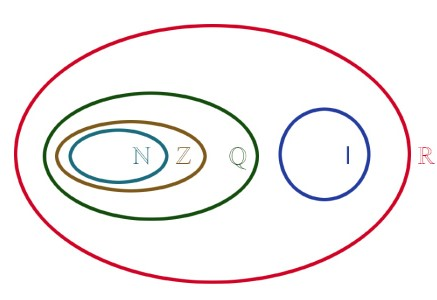
\includegraphics[width=10cm]{imagens/relação.jpg}
        \end{center}
        \begin{center}
            
        \end{center}
    \end{frame}
    
    % Slide 9
    \begin{frame}
        \begin{center}
            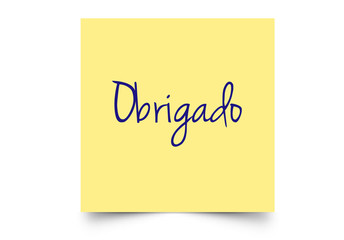
\includegraphics[width=5cm]{imagens/obrigado.jpg}
        \end{center}
        \begin{center}
            \textbf{Provérbios 1:7.a}
        \end{center}
        \begin{center}
            "O temor do Senhor é o princípio da ciência."
        \end{center}
    \end{frame}
\end{document}
